\documentclass[10pt, twocolumn, twoside, letterpaper]{IEEEtran}

\usepackage[activate={true, nocompatibility}, final, tracking=true, kerning=true, spacing=true, factor=1100, stretch=10, shrink=10]{microtype}
\linespread{0.9}

%\def\mycopyrightnotice{
%  {\footnotesize
%  \begin{minipage}{\textwidth}
%  \centering
%  {978-1-7281-4164-0/19/\$31.00 \copyright2019 IEEE
%  \end{minipage}
%  }
%}

\makeatletter
\def\ps@IEEEtitlepagestyle{
  %\def\@oddfoot{\mycopyrightnotice}
  \def\@evenfoot{}
}

\ifCLASSINFOpdf
   \usepackage[pdftex]{graphicx}
\else
   \usepackage[dvips]{graphicx}
\fi

\ifCLASSOPTIONcompsoc
  \usepackage[caption=false, font=normalsize, labelfont=sf, textfont=sf]{subfig}
\else
  \usepackage[caption=false, font=footnotesize]{subfig}
\fi

\usepackage{amsmath}
\usepackage{bm}
\usepackage{amssymb}
\usepackage{algorithm}
\usepackage{algorithmic}
\usepackage{stfloats}
\usepackage{url}
\usepackage{siunitx}
\usepackage{fancyref}

\usepackage{geometry}
\geometry{letterpaper, top=0.7in, bottom=0.7in, left=0.65in, right=0.65in}

\usepackage[acronym, nomain]{glossaries}

% Define "long-s" key: 
\glsaddkey* {longs}% key 
{\glsentrylong{\glslabel}s}% default value 
{\glsentrylongs}% command analogous to \glsentrytext 
{\Glsentrylongs}% command analogous to \Glsentrytext 
{\glslongs}% command analogous to \glstext 
{\Glslongs}% command analogous to \Glstext 
{\GLSlongs}% command analogous to \GLStext

%% Define "short-s" key: 
\glsaddkey* {shorts}% key 
{\glsentryshort{\glslabel}s}% default value 
{\glsentryshorts}% command analogous to \glsentrytext 
{\Glsentryshorts}% command analogous to \Glsentrytext 
{\glsshorts}% command analogous to \glstext 
{\Glsshorts}% command analogous to \Glstext 
{\GLSshorts}% command analogous to \GLStext

\DeclareRobustCommand{\glss}[1]
{%
  \ifglsused{#1}{\glsshorts{#1}}{\glslongs{#1} (\glsshorts{#1})\glsunset{#1}}%
}

\DeclareRobustCommand{\Glss}[1]
{%
  \ifglsused{#1}{\Glsshorts{#1}}{\Glslongs{#1} (\glsshorts{#1})\glsunset{#1}}%
}

% Define "long-ing" key: 
\glsaddkey* {longing}% key 
{\glsentrylong{\glslabel}ing}% default value 
{\glsentrylonging}% command analogous to \glsentrytext 
{\Glsentrylonging}% command analogous to \Glsentrytext 
{\glslonging}% command analogous to \glstext 
{\Glslonging}% command analogous to \Glstext 
{\GLSlonging}% command analogous to \GLStext

%% Define "short-ing" key: 
\glsaddkey* {shorting}% key 
{\glsentryshort{\glslabel}ing}% default value 
{\glsentryshorting}% command analogous to \glsentrytext 
{\Glsentryshorting}% command analogous to \Glsentrytext 
{\glsshorting}% command analogous to \glstext 
{\Glsshorting}% command analogous to \Glstext 
{\GLSshorting}% command analogous to \GLStext

\DeclareRobustCommand{\glsing}[1]
{%
  \ifglsused{#1}{\glsshorting{#1}}{\glslonging{#1} (\glsshorting{#1})\glsunset{#1}}%
}

\DeclareRobustCommand{\Glsing}[1]
{%
  \ifglsused{#1}{\Glsshorting{#1}}{\Glslonging{#1} (\glsshorting{#1})\glsunset{#1}}%
}

% Define "long-ed" key: 
\glsaddkey* {longed}% key 
{\glsentrylong{\glslabel}ed}% default value 
{\glsentrylonged}% command analogous to \glsentrytext 
{\Glsentrylonged}% command analogous to \Glsentrytext 
{\glslonged}% command analogous to \glstext 
{\Glslonged}% command analogous to \Glstext 
{\GLSlonged}% command analogous to \GLStext

%% Define "short-ed" key: 
\glsaddkey* {shorted}% key 
{\glsentryshort{\glslabel}ed}% default value 
{\glsentryshorted}% command analogous to \glsentrytext 
{\Glsentryshorted}% command analogous to \Glsentrytext 
{\glsshorted}% command analogous to \glstext 
{\Glsshorted}% command analogous to \Glstext 
{\GLSshorted}% command analogous to \GLStext

\DeclareRobustCommand{\glsed}[1]
{%
  \ifglsused{#1}{\glsshorted{#1}}{\glslonged{#1} (\glsshorted{#1})\glsunset{#1}}%
}

\DeclareRobustCommand{\Glsed}[1]
{%
  \ifglsused{#1}{\Glsshorted{#1}}{\Glslonged{#1} (\glsshorted{#1})\glsunset{#1}}%
}

\newacronym{1D}{1D}{$1$-Dimensional}
\newacronym{2D}{2D}{$2$-Dimensional}
\newacronym{3D}{3D}{$3$-Dimensional}
\newacronym[longs={$3$-Dimensional Point Clouds}, shorts={3DPCs}]{3DPC}{3DPC}{$3$-Dimensional Point Cloud}
\newacronym{4D}{4D}{$4$-Dimensional}
\newacronym{4DCT}{4DCT}{$4$-Dimensional Computed Tomography}
\newacronym[longs={Attenuation Corrections}, shorts={ACs}, longing={Attenuation Correcting}, shorting={ACing}, longed={Attenuation Corrected}, shorted={ACed}]{AC}{AC}{Attenuation Correct}
\newacronym[longs={Affine Deformations}, shorts={ADs}, longing={Affine Deforming}, shorting={ADing}, longed={Affine Deformed}, shorted={ADed}]{AD}{AD}{Affine Deformation}
\newacronym{AP}{AP}{Anterior Posterior}
\newacronym{ATP}{ATP}{Adenosine Triphosphate}
\newacronym[longs={B-Splines}, shorts={BSs}, longing={B-Splining}, shorting={BSing}, longed={B-Splined}, shorted={BSed}]{BS}{BS}{B-Spline}
\newacronym[longs={Cross Correlations}, shorts={CCs}, longing={Cross Correlating}, shorting={CCing}, longed={Cross Correlated}, shorted={CCed}]{CC}{CC}{Cross Correlation}
\newacronym{CCP}{CCP}{Current Clinical Practise}
\newacronym{CCT}{CCT}{Cine Computed Tomography}
\newacronym{CG}{CG}{Conjugate Gradient}
\newacronym{COM}{COM}{Centre of Mass}
\newacronym[longs={Control Points}, shorts={CPs}]{CP}{CP}{Control Point}
\newacronym[longs={Control Point Grids}, shorts={CPGs}]{CPG}{CPG}{Control Point Grid}
\newacronym{CT}{CT}{Computed Tomography}
\newacronym{DD}{DD}{Data Driven}
\newacronym{DDG}{DDG}{Data Driven Gating}
\newacronym[longs={Deformation Vector Fields}, shorts={DVFs}]{DVF}{DVF}{Deformation Vector Field}
\newacronym{EANM}{EANM}{European Association of Nuclear Medicine}
\newacronym{EM}{EM}{Expectation Maximisation}
\newacronym{FDG}{FDG}{Fluorodeoxyglucose}
\newacronym{F-FDG}{F-FDG}{Fluorine-$18$ Fludeoxyglucose}
\newacronym[longs={Fields of View}, shorts={FOVs}]{FOV}{FOV}{Field Of View}
\newacronym{FWHM}{FWHM}{Full Width at Half Maximum}
\newacronym{GD}{GD}{Gradient Descent}
\newacronym{GE}{GE}{General Electric}
\newacronym[longs={Ground Truths}, shorts={GTs}]{GT}{GT}{Ground Truth}
\newacronym[longs={Hounsfield Units}, shorts={HUs}]{HU}{HU}{Hounsfield Unit}
\newacronym[longs={Image Registrations}, shorts={IRs}, longing={Image Registering}, shorting={IRing}, longed={Image Registered}, shorted={IRed}]{IR}{IR}{Image Registration}
\newacronym[longs={Kilo Becquerel per Millilitres}, shorts={KBq/mLs}]{KBq/mL}{KBq/mL}{Kilo Becquerel per Millilitre}
\newacronym[longs={Kilo Electron Volts}, shorts={KeVs}]{KeV}{KeV}{Kilo Electron Volt}
\newacronym[longs={Kilo Volt}, shorts={KVs}]{KV}{KV}{Kilo Volt}
\newacronym[longs={Light Emitting Diodes}, shorts={LEDs}]{LED}{LED}{Light Emitting Diode}
\newacronym[longs={Lines of Responce}, shorts={LORs}]{LOR}{LOR}{Line of Response}
\newacronym[longs={Mean Absolute Errors}, shorts={MAEs}]{MAE}{MAE}{Mean Absolute Error}
\newacronym{MAPE}{MAPE}{Mean Absolute Percentage Error}
\newacronym{MBF}{MBF}{Myocardial Blood Flow}
\newacronym[longs={Motion Compensated Image Reconstructions}, shorts={MCIRs}, longing={Motion Compensated Image Reconstructing}, shorting={MCIRing}, longed={Motion Compensated Image Reconstructed}, shorted={MCIRed}]{MCIR}{MCIR}{Motion Compensated Image Reconstruction}
\newacronym[longs={Motion Compensated Images}, shorts={MCIs}]{MCI}{MCI}{Motion Compensated Image}
\newacronym[longs={Motion Corrections}, shorts={MCs}, longing={Motion Correcting}, shorting={MCing} longed={Motion Corrected}, shorted={MCed}]{MC}{MC}{Motion Correction}
\newacronym{MI}{MI}{Mutual Information}
\newacronym{ML}{ML}{Maximum Likelihood}
\newacronym{MLAA}{MLAA}{Maximum Likelihood Reconstruction of Activity and Attenuation}
\newacronym{MLE}{MLE}{Maximum Likelihood Estimation}
\newacronym{MLEM}{MLEM}{Maximum Likelihood Expectation Maximisation}
\newacronym[longs={Motion Models}, shorts={MMs}, longing={Motion Modelling}, shorting={MMing}, longed={Motion Modelled}, shorted={MMed}]{MM}{MM}{Motion Model}
\newacronym[longs={Myocardial Perfusion Images}, shorts={MPIs}, longing={Myocardial Perfusion Imaging}, shorting={MPIing}, longed={Myocardial Perfusion Imaged}, shorted={MPIed}]{MPI}{MPI}{Myocardial Perfusion Image}
\newacronym{MR}{MR}{Magnetic Resonance}
\newacronym[longs={Mean Squared Errors}, shorts={MSEs}]{MSE}{MSE}{Mean Squared Error}
\newacronym[longs={Attenuation Maps}, shorts={Mu-Maps}]{Mu-Map}{Mu-Map}{Attenuation Map}
\newacronym[longs={Non-Attenuation Corrections}, shorts={NACs}, longing={Non-Attenuation Correcting}, shorting={NACing}, longed={Non-Attenuation Corrected}, shorted={NACed}]{NAC}{NAC}{Non-Attenuation Correct}
\newacronym{NMI}{NMI}{Normalised Mutual Information}
\newacronym{ND}{ND}{$n$-Dimensional}
\newacronym[longs={Non-Rigid Deformations}, shorts={NRDs}, longing={Non-Rigid Deforming}, shorting={NRDing}, longed={Non-Rigid Deformed}, shorted={NRed}]{NRD}{NRD}{Non-Rigid Deformation}
\newacronym{NTOF}{NTOF}{Non-Time of Flight}
\newacronym{OSEM}{OSEM}{Ordered Subset Expectation Maximisation}
\newacronym[longs={Principal Components}, shorts={PCs}]{PC}{PC}{Principal Component}
\newacronym{PCA}{PCA}{Principal Component Analysis}
\newacronym{PET}{PET}{Positron Emission Tomography}
\newacronym{PSMA}{PSMA}{Prostate Specific Membrane Antigen}
\newacronym[longs={Respiratory Correspondence Models}, shorts={RCMs}, longing={Respiratory Correspondence Modelling}, shorting={RCMing}, longed={Respiratory Correspondence Modelled}, shorted={RCMed}]{RCM}{RCM}{Respiratory Correspondence Model}
\newacronym[longs={Rigid Deformations}, shorts={RDs}, longing={Rigid Deforming}, shorting={RDing}, longed={Rigid Deformed}, shorted={RDed}]{RD}{RD}{Rigid Deformation}
\newacronym{RDP}{RDP}{Relative Difference Prior}
\newacronym[longs={Respiratory Motions}, shorts={RMs}]{RM}{RM}{Respiratory Motion}
\newacronym[longs={Regions of Interest}, shorts={ROIs}]{ROI}{ROI}{Region of Interest}
\newacronym{RPM}{RPM}{Real Time Position Management}
\newacronym{SGD}{SGD}{Stochastic Gradient Descent}
\newacronym{SI}{SI}{Superior Inferior}
\newacronym{SIRF}{SIRF}{Synergistic Image Reconstruction Framework}
\newacronym[longs={Signal to Noise Ratios}, shorts={SNRs}]{SNR}{SNR}{Signal to Noise Ratio}
\newacronym[longs={Surrogate Signals}, shorts={SSs}]{SS}{SS}{Surrogate Signal}
\newacronym{SSD}{SSD}{Sum of Squared Differences}
\newacronym{STIR}{STIR}{Software for Tomographic Image Reconstruction}
\newacronym[longs={Standard Uptake Values}, shorts={SUVs}]{SUV}{SUV}{Standard Uptake Value}
\newacronym{SVD}{SVD}{Singular Value Decomposition}
\newacronym{TOF}{TOF}{Time of Flight}
\newacronym[longs={Thin Plate Splines}, shorts={TPSs}]{TPS}{TPS}{Thin Plate Spline}
\newacronym{XCAT}{XCAT}{$4$-Dimensional Extended Cardiac Torso}


\newcommand{\cmmnt}[1]{\@bsphack\@esphack}

\usepackage[style=ieee, doi=false, isbn=false, url=false, maxbibnames=1, minbibnames=1, maxcitenames=1, mincitenames=1, backend=biber, defernumbers=false]{biblatex}
\addbibresource{./bibtex/bib/Biblio.bib}

%\IEEEpubid{\begin{minipage}{\textwidth}\ \\[9pt] \centering
%\medskip
%\\
%978-1-7281-2260-1/19/\$31.00~\copyright~2019~IEEE
%\end{minipage}}

\begin{document}
\title{Extension of Static PCA Based Data Driven Surrogate Signal Extraction Methods to Dynamic PET Using Moving Windows and Eigenvector Backpropergation}

\pagestyle{plain}
\pagenumbering{gobble}

\author{Alexander~C.~Whitehead,~\IEEEmembership{Student~Member,~IEEE,}
        Elise~C.~Emond
        Kuan-Hao~Su
        Ander~Biguri
        Joanna~C.~Porter
        Helen~Garthwaite
        Maria?
        Scott~W.~Wollenweber,~\IEEEmembership{Senior~Member~IEEE,}
        Charles~W.~Stearns,~\IEEEmembership{Fellow,~IEEE,}
        Brian~F.~Hutton,~\IEEEmembership{Senior~Member,~IEEE,}
        Jamie~R.~McClelland
        and~Kris~Thielemans,~\IEEEmembership{Senior~Member,~IEEE}%

    \thanks{Alexander~C.~Whitehead, Brian~F.~Hutton and Kris~Thielemans are with the Institute of Nuclear Medicine, University College London, London, NW1~2BU, UK (contact: \texttt{alexander.whitehead.18@ucl.ac.uk}).}%
    \thanks{Alexander~C.~Whitehead and Jamie~R.~McClelland are with the Centre for Medical Image Computing, University College London, London, NW1~2BU, UK.}%
    \thanks{Scott~Wollenweber and Charles~Stearns are with Molecular Imaging \& Computed Tomography Engineering, GE Healthcare, USA}%
    \thanks{This research is supported by GE Healthcare, the NIHR UCLH Biomedical Research Centre and the EPSRC-funded UCL Centre for Doctoral Training in Medical Imaging (EP/L016478/1). The software used was partly produced by the Computational Collaborative Project in Synergistic PET-MR Reconstruction, CCP PET-MR, UK EPSRC grant EP/M022587/1 and the CCP on Synergistic Biomedical Imaging, CCP SyneRBI, UK EPSRC grant EP/T026693/1}%
    \thanks{Jamie~R.~McClelland is supported by a Cancer Research UK Centres Network Accelerator Award Grant (A21993) to the ART-NET consortium and a CRUK Multi-disciplinary grant (CRC 521).}%
}

\maketitle
\IEEEpeerreviewmaketitle

\begin{abstract}
    
\end{abstract}

\section{Introduction} \label{sec:introduction}
    \IEEEPARstart{R}{espiratory} motion reduces image resolution in \gls{PET} by introducing blurring \& mis-alignment artefacts~\cite{Nehmeh2008a}. This is often combated through the use of gated reconstruction and motion correction. A weakness of gated reconstruction is that it requires a \gls{SS} which reflects the respiratory position of the patient over the acquisition. Methods to determine \glss{SS} include those which use an external device, like the \gls{RPM}, a disadvantage of these methods are that they require the use of additional equipment and a change to clinical practise. Thus, \gls{DD} methods to extract \glss{SS} have become an alternative, these include \gls{PCA}~\cite{Thielemans2011}.
    
    A disadvantage of \gls{DD} \gls{SS} extraction methods are that they often do not work for dynamic \gls{PET} data where the tracer kinetics offer more variance than the \gls{RM} does. Previously a moving window method using \gls{FDA} was proposed~\cite{Schleyer2014}. This work seeks to implement a moving window method using \gls{PCA} and then compare this to static \gls{PCA} and other \gls{PCA} based dynamic \gls{DD} \gls{SS} extraction methods.

\section{Methods} \label{sec:methods}
\subsection{Data Acquisition} \label{sec:data_acquisition}
        Seven dynamic \gls{FDG} acquisitions, with a \gls{FOV} covering the upper lung \& heart, were acquired on a \gls{GE} Discovery $710$. Each acquisition lasted approximately \SI{20}{\minute} with the acquisition starting before injection of the radiotracer. \gls{SS} were acquired in parallel using a \gls{RPM}.
        
    \subsection{Data Preparation} \label{sec:data_preparation}
        Data were unlisted into low resolution sinograms, at a time interval of \SI{500}{\milli\second}, using the \gls{GE} PetToolbox following~\cite{Bertolli2018Data-DrivenTomography}. Data was preprocessed by removing the first \& last element in the axial direction \& applying a Freeman-Tukey to stabilise the variance of the Poisson data. The Freeman-Tukey transformation is defined as:
        
        \begin{equation}
            S = 2 \sqrt{S + \frac{3}{8}}
        \end{equation}
        
        \noindent $S$ is the resultant sinogram of applying the Freeman-Tukey transformation to sinogram $S$~\cite{Freeman1950TransformationsRoot}.
    
    \subsection{Surrogate Signal Extraction} \label{sec:surrogate_signal_extraction}
        \subsubsection{Moving Window} \label{sec:moving_window}
            This method takes data window by window (with half a window overlap) \& extracts a \gls{SS} using \gls{PCA}. The final \gls{SS} is constructed by determining the sign of the current \gls{SS}, flipping it if necessary, \& then concatenating it with the next. The size of the window increases as the acquisition goes on. Motivation is that at early time points the variation caused by the tracer kinetics obscures that which comes from respiratory motion, if the window is smaller than the period of the tracer kinetics then it should obtain the respiratory \gls{SS}.
        
        \subsubsection{One \gls{PC}} \label{sec:one_pc}
            This method takes late time point \glss{PC} \& applies them to early time point data. Motivation is that the \glss{PC} of late time point data do not vary significantly, therefore it could be assumed that the variation of early time point \glss{PC} are caused mostly by the tracer kinetics.
        
        \subsubsection{Joint Method} \label{sec:joint_method}
            This method attempts to take the advantages of both the one \gls{PC} method \& the static method, by truncating \& concatenating the result of the start of one with the end of the other. Motivation is that the static method would work better on static data, once the tracer kinetics have subsided the acquisition could be considered to be static.
    
    
    \subsection{Evaluation} \label{sec:evaluation}
        \subsubsection{Cross Correlation} \label{sec:cross_correlation}
            The \gls{CC} of each \gls{SS} between each method \& the \gls{RPM}, for all acquisitions, has been calculated. Additionally, the early time point \glss{SS} for each method have been plotted against the \gls{RPM}, for the first acquisition.
        
        \subsubsection{Reconstruction} \label{sec:reconstruction}
            Data has been reconstructed, for the first acquisition, using each \gls{SS} to displacement gate the data into $10$ bins. Reconstructions were performed using \gls{GE} Duetto using \gls{TOF} \gls{OSEM} with two full iterations \& $24$ subsets.%~\cite{Hudson1994}.
            Volumes were post-filtered using a Gaussian blur with a kernel size of \SI{6.4}{\milli\metre} \gls{FWHM}.
            
            Comparisons between these \gls{MC} reconstructed volumes includes: A profile over the aorta \& \gls{SUV}\textsubscript{max}, \gls{SUV}\textsubscript{median} \& \gls{SUV}\textsubscript{peak}. \gls{SUV}\textsubscript{peak} here was defined following \gls{EANM} guidelines.%~\cite{Boellaard2015FDG2.0}
        
\section{Results} \label{sec:results}
    \begin{table}
        \centering
        \captionsetup{singlelinecheck=false, justification=centering}
        \caption{A comparison of the \gls{CC} between the \gls{RPM} \gls{SS} \& the \gls{SS} from the static \gls{PCA}, the moving window, the one \gls{PC} \& the joint methods for $7$ acquisitions.}
        
        \resizebox*{0.75\linewidth}{!}
        {
            \begin{tabular}{||c|cccc||}
                \hline
                \textbf{\gls{CC}} & \textbf{Static \gls{PCA}} & \textbf{Moving Window} & \textbf{One \gls{PC}} & \textbf{Joint Method} \\
                \hline
                \textbf{Acquisition $1$}   & $0.0387$  & $0.486$  & $0.565$  & $0.493$   \\
                \textbf{Acquisition $2$}   & $0.0985$  & $0.0361$ & $0.281$  & $0.0227$  \\
                \textbf{Acquisition $3$}   & $0.00797$ & $0.0388$ & $0.224$  & $0.00459$ \\
                \textbf{Acquisition $4$}   & $0.242$   & $0.0467$ & $0.273$  & $0.0946$  \\
                \textbf{Acquisition $5$}   & $0.0759$  & $0.793$  & $0.819$  & $0.798$   \\
                \textbf{Acquisition $6$}   & $0.0594$  & $0.246$  & $0.363$  & $0.259$   \\
                \textbf{Acquisition $7$}   & $0.160$   & $0.629$  & $0.203$  & $0.526$   \\
                \hline
            \end{tabular}
        }
        \label{tab:cross_correlation}
    \end{table}
    
    A comparison of \gls{CC} can be seen in in~\Fref{tab:cross_correlation}. The results for the moving window method show that it usually performs better than static \gls{PCA}, a reason why these results may be varied is because the hyper parameters for this method were optimised for one acquisition. The results for the one \gls{PC} method are consistently better than the static \gls{PCA} method.
    
    \begin{figure}
        \centering
        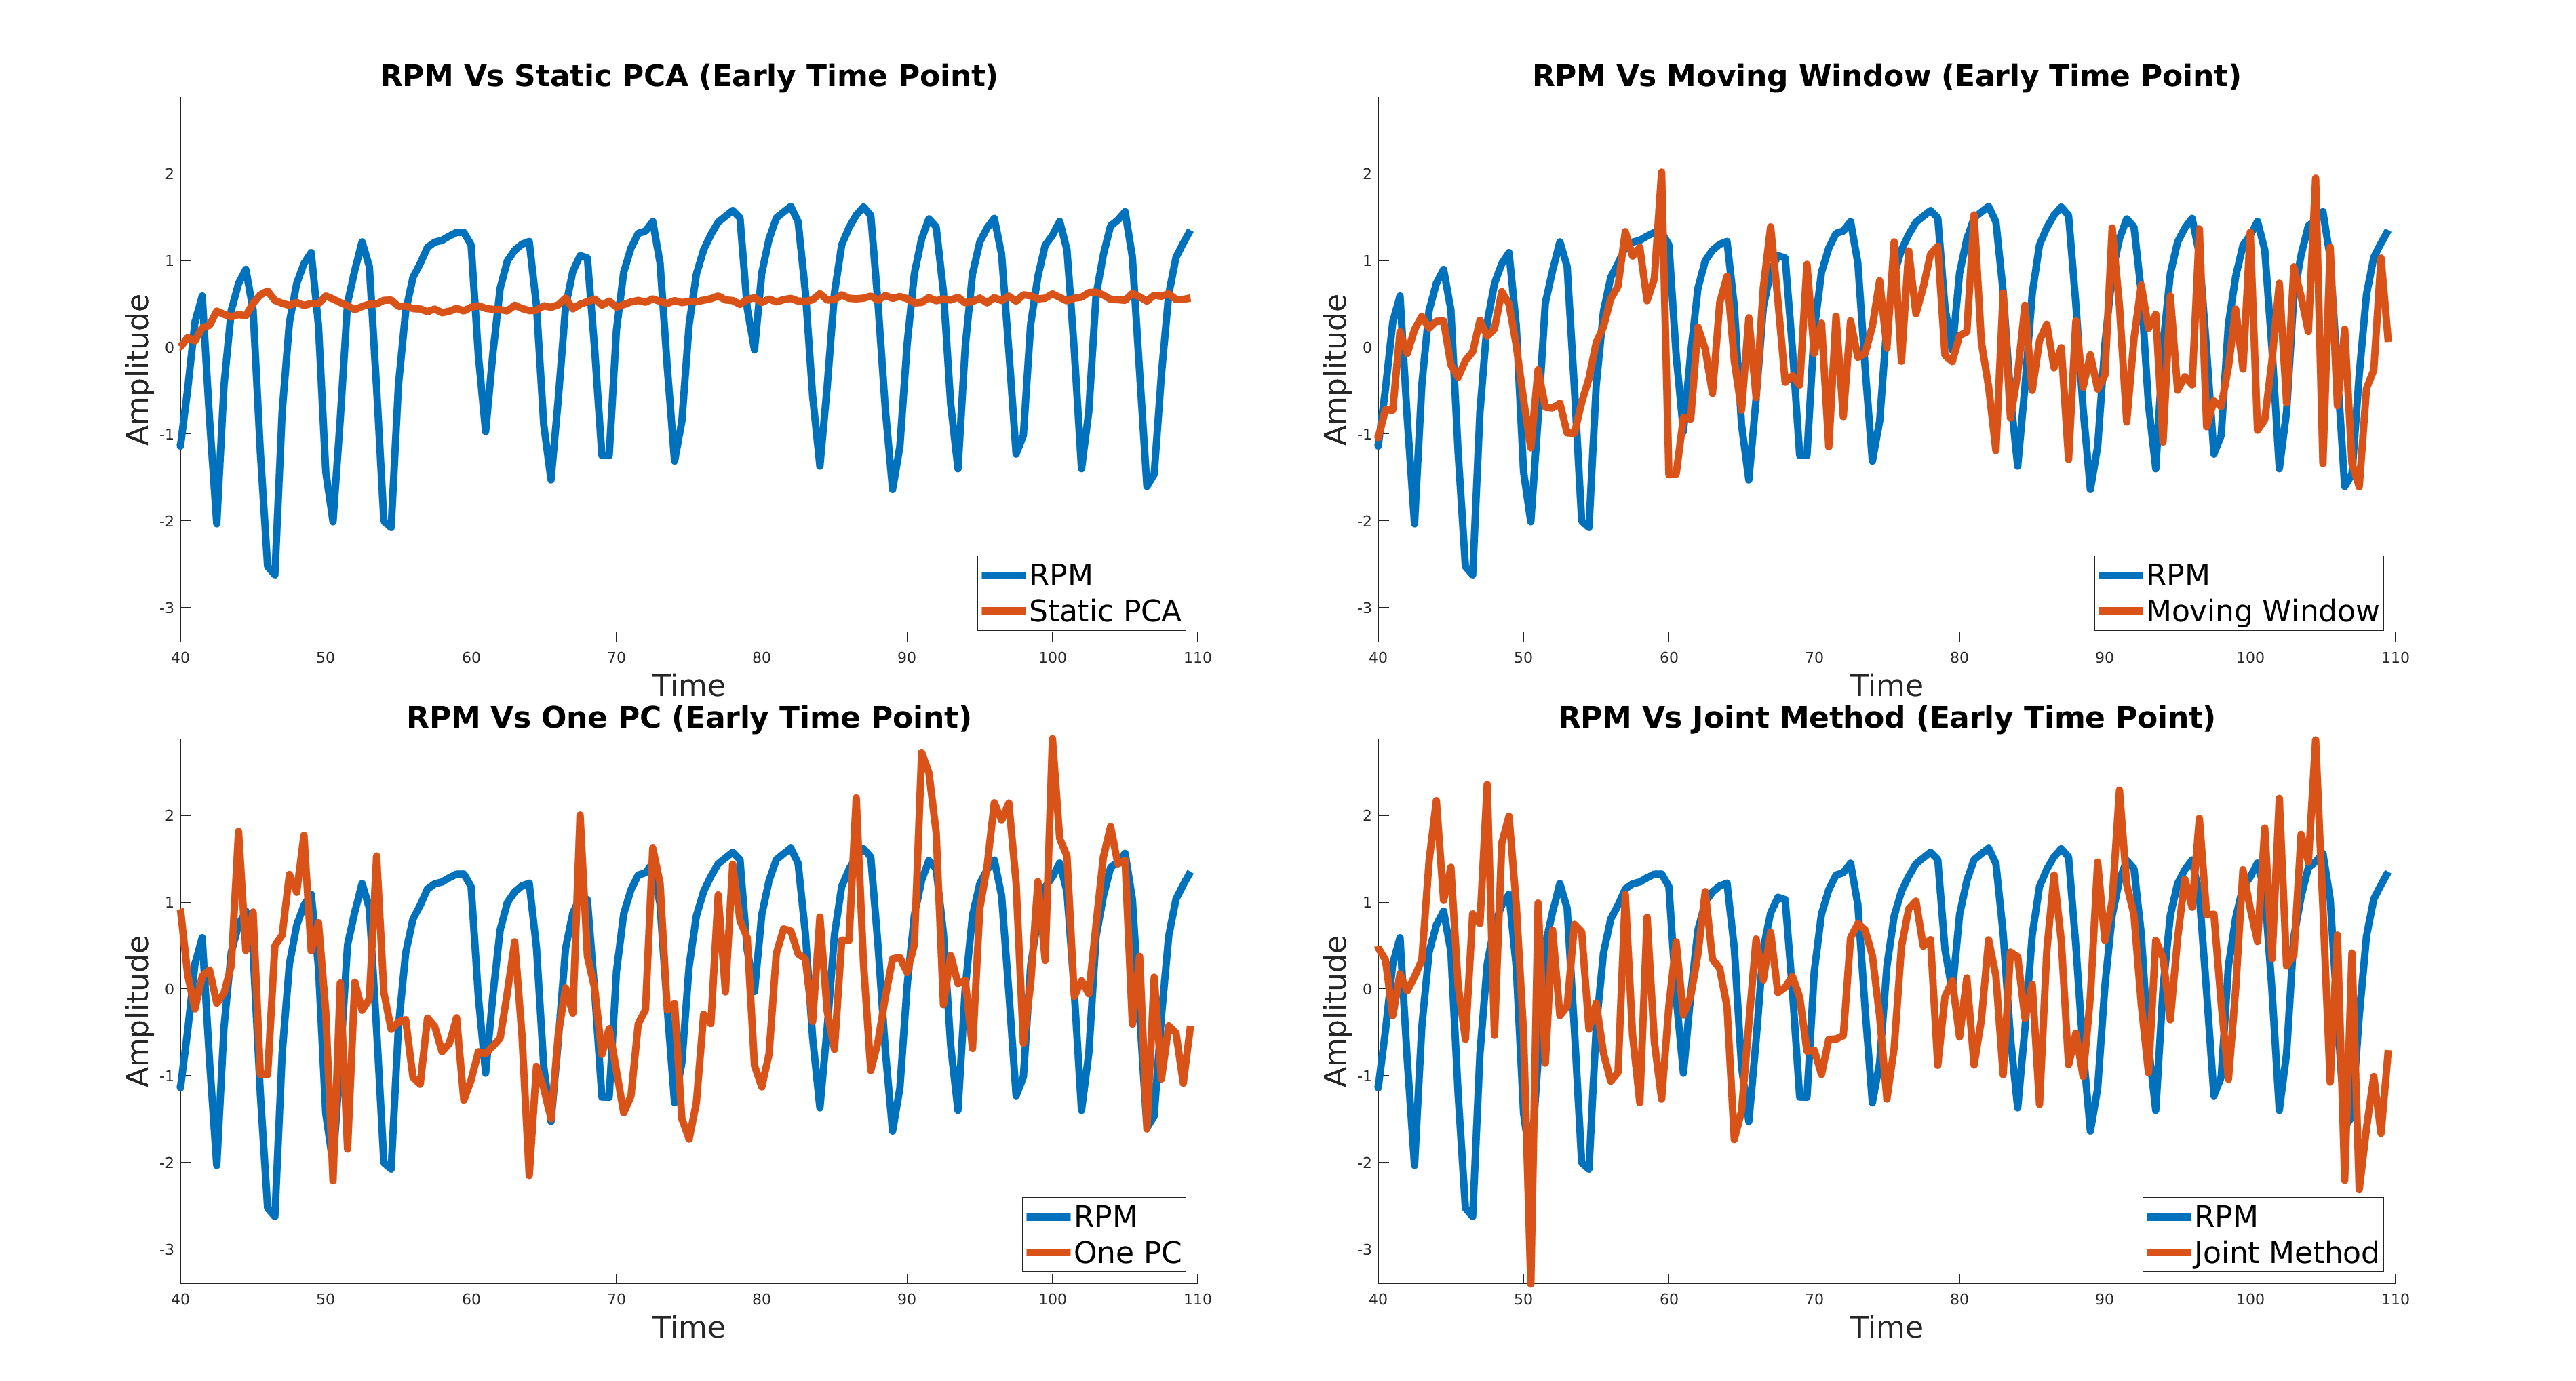
\includegraphics[width=1.0\linewidth]{figures/surrogate_signal.png}
        \captionsetup{singlelinecheck=false, justification=centering}
        \caption{A comparison between the \gls{RPM} \gls{SS} \& the \gls{SS} from the static \gls{PCA}, the moving window, the one \gls{PC} \& the joint methods.}
        \label{fig:surrogate_signal}
    \end{figure}
    
    \begin{figure}
        \centering
        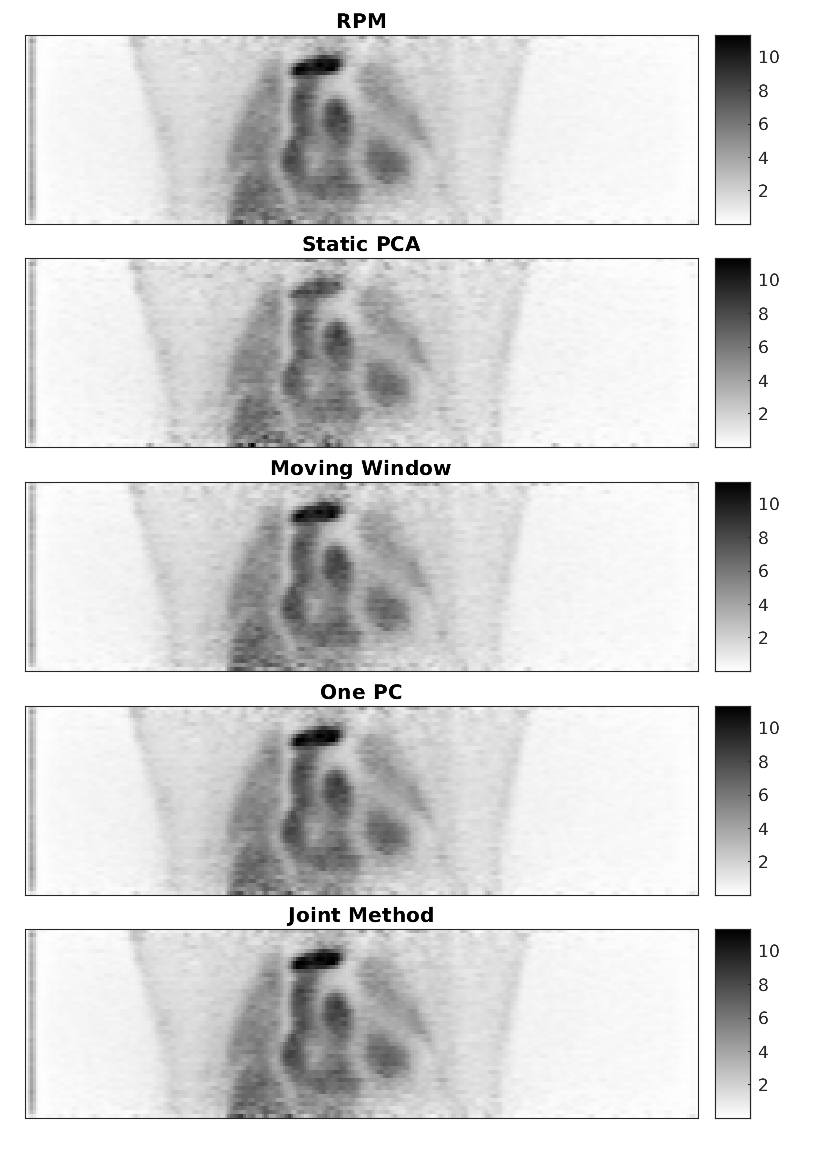
\includegraphics[width=0.75\linewidth]{figures/visual_analysis_pca.png}
        \captionsetup{singlelinecheck=false, justification=centering}
        \caption{Gated reconstructions using \gls{RPM}, static \gls{PCA} method, moving window method, one \gls{PC} method \& joint method. Colour map ranges are consistent for all images.}
        \label{fig:visual_analysis}
    \end{figure}
    
    \begin{figure}
        \centering
        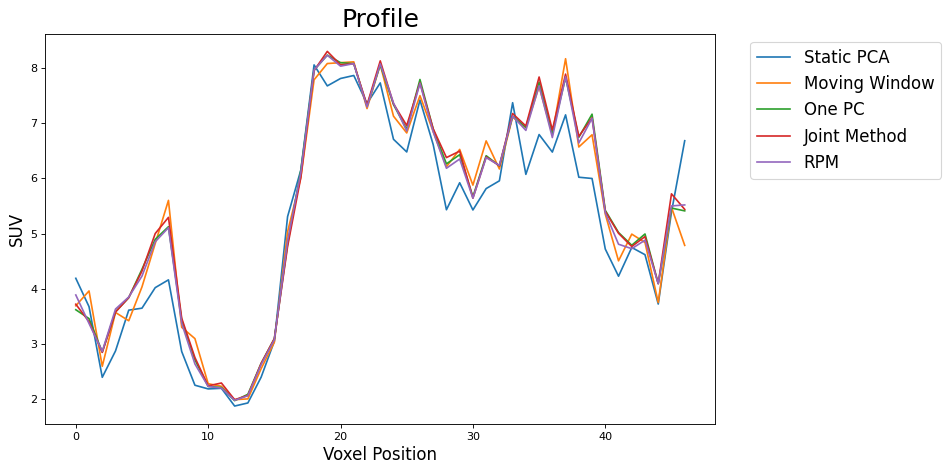
\includegraphics[width=0.5\linewidth]{figures/profile_pca.png}
        \captionsetup{singlelinecheck=false, justification=centering}
        \caption{A profile across the aorta for gated reconstructions using \gls{RPM}, static \gls{PCA} method, moving window method, one \gls{PC} method \& joint method.}
        \label{fig:profile}
    \end{figure}
    
    \begin{table}
        \centering
        \captionsetup{singlelinecheck=false, justification=centering}
        \caption{Comparison of \gls{SUV}\textsubscript{max}, \gls{SUV}\textsubscript{median} \& \gls{SUV}\textsubscript{peak} between gated reconstructions using \gls{RPM}, static \gls{PCA} method, moving window method, one \gls{PC} method \& joint method.}
        
        \resizebox*{0.5\linewidth}{!}
        {
            \begin{tabular}{||c|ccc||}
                \hline
                \textbf{\gls{SUV}} & \textbf{Max} & \textbf{Median} & \textbf{Peak} \\
                \hline
                \textbf{\gls{RPM}}          & $18.4$ & $10.9$ & $12.6$ \\
                \hline
                \textbf{Static \gls{PCA}}   & $12.8$ & $10.6$ & $11.4$ \\
                \textbf{Moving Window}      & $14.5$ & $10.6$ & $11.3$ \\
                \textbf{One \gls{PC}}       & $18.5$ & $10.9$ & $12.6$ \\
                \textbf{Joint Method}       & $18.5$ & $11.0$ & $12.8$ \\
                \hline
            \end{tabular}
        }
        \label{tab:suv}
    \end{table}
    
    A plot of the \gls{SS} for all methods can be seen in~\Fref{fig:surrogate_signal}, the one \gls{PC} method matches the \gls{RPM} best in this example. The reconstructed data, using \glss{SS} from all methods can be seen in~\Fref{fig:visual_analysis}, the clarity of the reconstruction around the aorta seems diminished in the static \gls{PCA} example, it is similar in all other examples. A profile across the aorta can be seen in~\Fref{fig:profile}, this shows that the static \gls{PCA} method differs in its distribution. \gls{SUV} results can be seen in~\Fref{tab:suv} \& show that \glss{SUV} are consistent with \gls{RPM} for both the one \gls{PC} method \& the joint method.
    
\section{Discussion \& Conclusions} \label{sec:discussion_and_conclusions}
    Results from a comparison of \gls{CC}, a comparison of profiles \& \glss{SUV} show that the one \gls{PC} and joint method show promise in \gls{DD} extraction of \gls{SS} from dynamic data when compared to the static method.
    
    In the future, research will focus on further development of the one \gls{PC} method, including tuning its hyper parameters as well as testing it on a wider array of data.


\AtNextBibliography{\scriptsize}
\printbibliography

\end{document}
